\documentclass[t, aspectratio=169]{beamer}
\usepackage[utf8]{vietnam}
\usepackage{amsthm,amsmath,amssymb}
\usepackage{lmodern}

% --- CẤU HÌNH LỀ ---
\def\slideContentLeftMargin{0.5cm}
\def\slideContentRightMargin{1cm}
\def\hustHeaderHeight{1cm}
\def\slideContentBotMargin{3.5cm}

\usepackage[blue, 169]{beamerthemeHUST}
\graphicspath{{hust_theme/images/}{figures/}}

% Vị trí khối title ở trang title
\renewcommand{\titlePageTitleX}{-0.5cm}
\renewcommand{\titlePageTitleY}{-0.5cm}
\renewcommand{\hustTitleAlign}{\alignLeft}
\renewcommand{\hustSubtitleAlign}{\alignLeft}
\renewcommand{\hustAuthorAlign}{\alignLeft}
\renewcommand{\hustInstAlign}{\alignLeft}

\title{HỖN LOẠN VÀ ĐIỀU KHIỂN LỊCH TRÌNH XE BUÝT CON THOI}
\subtitle{Một nghiên cứu hệ động lực dựa trên Nagatani (2006)}
\author{\texorpdfstring{Nhóm 3 -- Người A, Người B, Người C}{Nhom 3 - Nguoi A, Nguoi B, Nguoi C}}
\institute{Mô hình hóa toán học -- Đại học Bách khoa Hà Nội}

\begin{document}

\hustintropage{\\[3.2cm] Mô hình hóa hỗn loạn\\trong hệ thống xe buýt con thoi}

\husttitlepage

\begin{frame}{Nội dung trình bày}
	\tableofcontents
\end{frame}

\resetPageCount
\showPageNumber

\useStyleHustFull
\useThinBar

% =====================================================================
\section{Mở đầu}
% =====================================================================

\begin{frame}{1. Bài toán dồn xe (Bus Bunching)}
	\textbf{Một hiện tượng quen thuộc:}
	\begin{itemize}
		\item Một xe buýt con thoi chạy khứ hồi giữa hai điểm, không có thời gian biểu cố định.
		\item Thời gian một chuyến phụ thuộc vào \textbf{số khách} đón được, và số khách lại phụ thuộc vào \textbf{khoảng cách thời gian} với xe trước (headway).
		\item Phản hồi vòng này có thể khiến các xe \emph{dồn lại thành cụm} -- xe ban đầu cách đều nhau, dần dần lệch nhịp rồi dồn lại với nhau.
	\end{itemize}

	\vspace{0.7em}
	\textbf{Câu hỏi nghiên cứu:} khi một tham số duy nhất -- mức độ "tải" của lịch trình -- tăng lên, khi nào hệ \textbf{ổn định}, khi nào trở nên \textbf{tuần hoàn}, khi nào \textbf{hỗn loạn}, và khi nào \textbf{sụp đổ hoàn toàn}?
\end{frame}

% =====================================================================
\section{Mô hình}
% =====================================================================

\begin{frame}{2. Phương trình chủ đạo}
	Gọi $t_i(m)$ là thời điểm xe $i$ khởi hành ở chuyến thứ $m$:
	\begin{equation}
		t_i(m+1) = t_i(m) + (\gamma + \eta)\, B_i(m) + \frac{2L}{V_i(m)}, \qquad i = 1,\dots,M
	\end{equation}

	\vspace{0.3em}
	\begin{itemize}
		\item $B_i(m) = \mu\,\big(t_i(m) - t_{i'}(m')\big)$: số khách lên xe $i$, tỉ lệ với \textbf{headway} so với xe trước.
		\item $(\gamma+\eta)$: thời gian lên/xuống xe trung bình mỗi khách.
		\item $V_i(m) = V_0 + s_i (\gamma+\eta) B_i(m)$: \textbf{tốc độ tăng theo lượng khách} -- xe đông thì chạy nhanh hơn để bù thời gian.
		\item $2L$: quãng đường khứ hồi của tuyến.
	\end{itemize}

	\vspace{0.3em}
	$\Rightarrow$ Headway nhỏ $\to$ ít khách $\to$ xe chạy chậm hơn $\to$ headway lại thay đổi ở vòng sau: một \textbf{hệ động lực phi tuyến, lặp}.
\end{frame}

\begin{frame}{3. Bản đồ phi tuyến cho hai xe}
	Đổi thang thời gian và nhóm các hằng số,
	\[
		T_i \equiv t_i \cdot \frac{V_0}{2L}, \qquad
		\Gamma \equiv \mu(\gamma+\eta), \qquad
		S_i \equiv s_i\,\mu(\gamma+\eta)\cdot\frac{2L}{V_0^2},
	\]
	phương trình chủ đạo trở thành một \textbf{bản đồ không thứ nguyên} gọn gàng:
	\begin{equation}
		T_i(m+1) = T_i(m) + \Gamma \cdot H_i(m) + \frac{1}{1 + S_i \cdot H_i(m)},
		\qquad H_i(m) \equiv T_i(m) - T_{i'}(m')
	\end{equation}

	\begin{itemize}
		\item $H_i(m)$: \textbf{headway} -- khoảng thời gian giữa xe $i$ và xe trước nó.
		\item $\Gamma$: \textbf{tham số tải} -- mức độ lượng khách làm chậm xe.
		\item $S_i$: \textbf{tham số tăng tốc} -- mức độ xe $i$ bù lại bằng cách chạy nhanh hơn.
	\end{itemize}

	\alert{Toàn bộ động lực học của hệ chỉ phụ thuộc vào hai đại lượng: $\Gamma$ và $\{S_i\}$.}
\end{frame}

\begin{frame}{4. Tính ổn định \& ngưỡng phân kỳ}
	Với 2 xe đối xứng ($S_1=S_2=S$), giả sử hệ tiến tới headway không đổi $\Delta$:
	\[
		\Delta = \Gamma\Delta + \frac{1}{1+S\Delta}
		\;\;\Longleftrightarrow\;\;
		(1-\Gamma)\,\Delta\,(1+S\Delta) = 1.
	\]

	\begin{itemize}
		\item Với $\Gamma < 1$: tồn tại nghiệm dương $\Delta^*$ -- hệ tiến tới một headway ổn định (\textbf{regular motion}).
		\item Khi $\Gamma \to 2$: phương trình không còn nghiệm dương hợp lệ $\Rightarrow$ \textbf{tour-time tăng không giới hạn -- hệ sụp đổ}.
		\item Giữa hai cực đó là một \textbf{đường chuyển pha} ngăn cách regular motion với periodic/chaotic motion:
		\[
			\Gamma^* = \frac{S}{S+1} \qquad (\text{với } S_1=S_2=S).
		\]
	\end{itemize}

	\small Quan hệ này được kiểm chứng số ở Fig. 8 và khớp với giá trị Nagatani đã công bố.
\end{frame}

% =====================================================================
\section{Phương pháp}
% =====================================================================

\begin{frame}{5. Mô phỏng động lực học của hệ xe buýt}
	\textbf{Điểm tinh tế:} xe có thể \emph{vượt nhau}, nên "xe trước" trong $H_i(m)$ \textbf{không cố định trước} -- nó phụ thuộc vào chính diễn biến của hệ.

	\vspace{0.5em}
	\textbf{Cách tiếp cận -- mô phỏng event-driven:}
	\begin{enumerate}
		\item Theo dõi thời điểm khởi hành tiếp theo của mỗi xe trên một dòng thời gian.
		\item Ở mỗi bước, cho xe sắp khởi hành sớm nhất tiến lên.
		\item Headway của nó được đo so với xe khởi hành ngay trước nó theo thời gian thực -- không phải một "đối tác" gán sẵn.
		\item Áp dụng bản đồ để tính thời điểm khởi hành tiếp theo, rồi lặp lại.
	\end{enumerate}

	\vspace{0.5em}
	Sau khi bỏ qua một đoạn transient ban đầu, phần quỹ đạo còn lại cho ta hành vi ổn định dài hạn dùng trong toàn bộ kết quả tiếp theo.
\end{frame}

% =====================================================================
\section{Kết quả: Chuỗi thời gian}
% =====================================================================

\begin{frame}{6. Động lực học của headway}
	\begin{columns}[T]
		\begin{column}{0.5\textwidth}
			\centering
			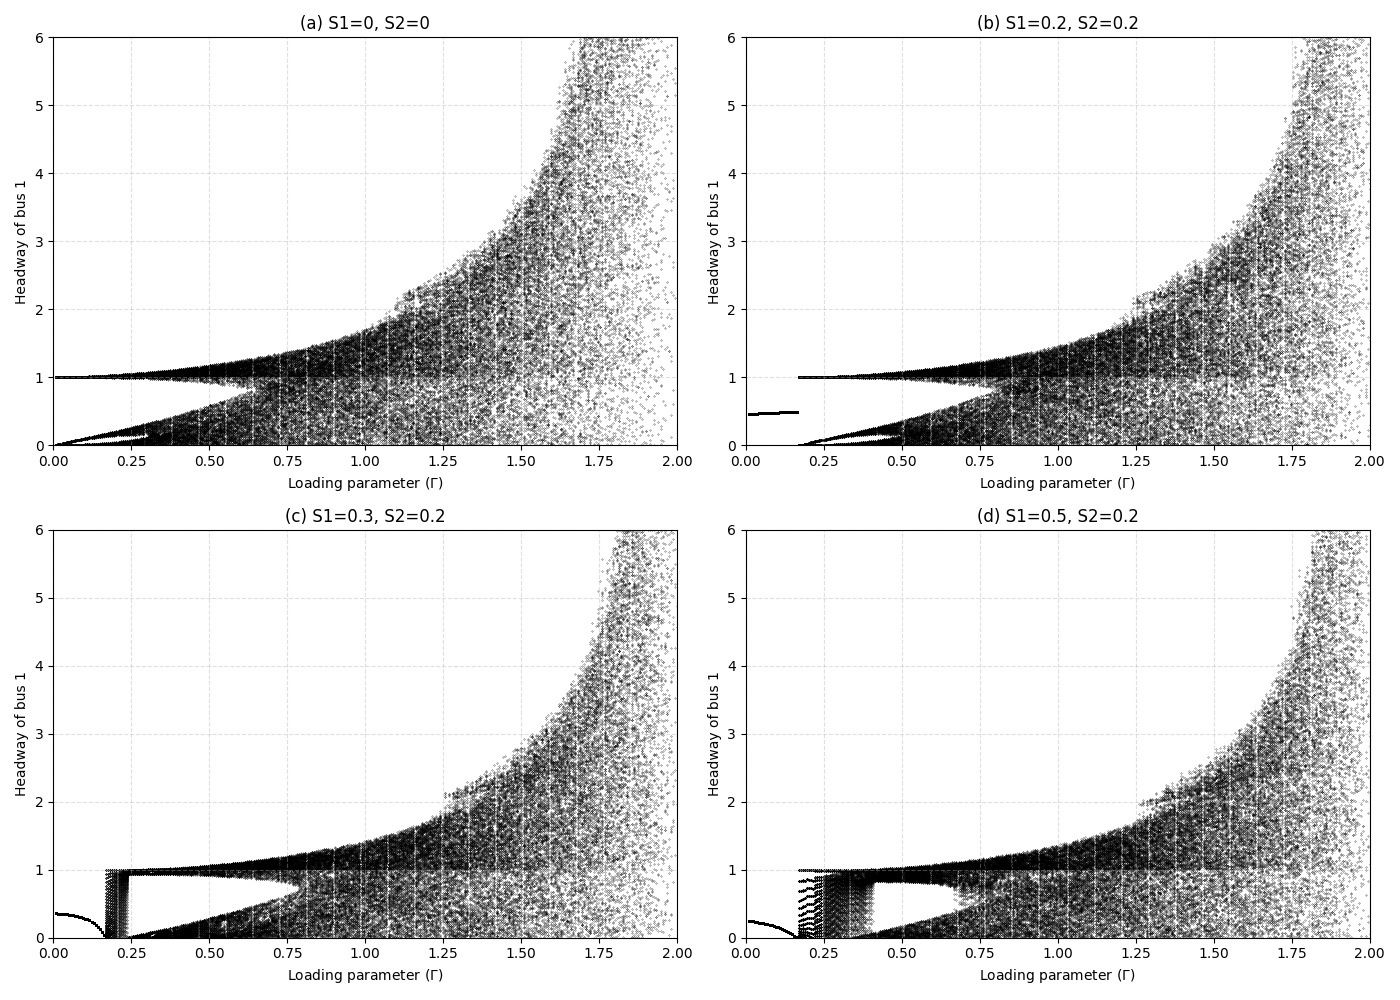
\includegraphics[width=\textwidth]{fig2_time_headway.png}
		\end{column}
		\begin{column}{0.5\textwidth}
			\centering
			
\includegraphics[width=\textwidth]{fig3_zoom.png}
		\end{column}
	\end{columns}

	\vspace{0.5em}
	Với $\Gamma$ nhỏ, headway của 2 xe nhanh chóng hội tụ về một giá trị cố định (\textbf{regular motion}). Khi $\Gamma$ tăng dần qua $\Gamma^*$, headway bắt đầu dao động \textbf{tuần hoàn}, rồi \textbf{hỗn loạn}.
\end{frame}

\begin{frame}{7. Động lực học của tour-time}
	\begin{columns}[T]
		\begin{column}{0.5\textwidth}
			\centering
			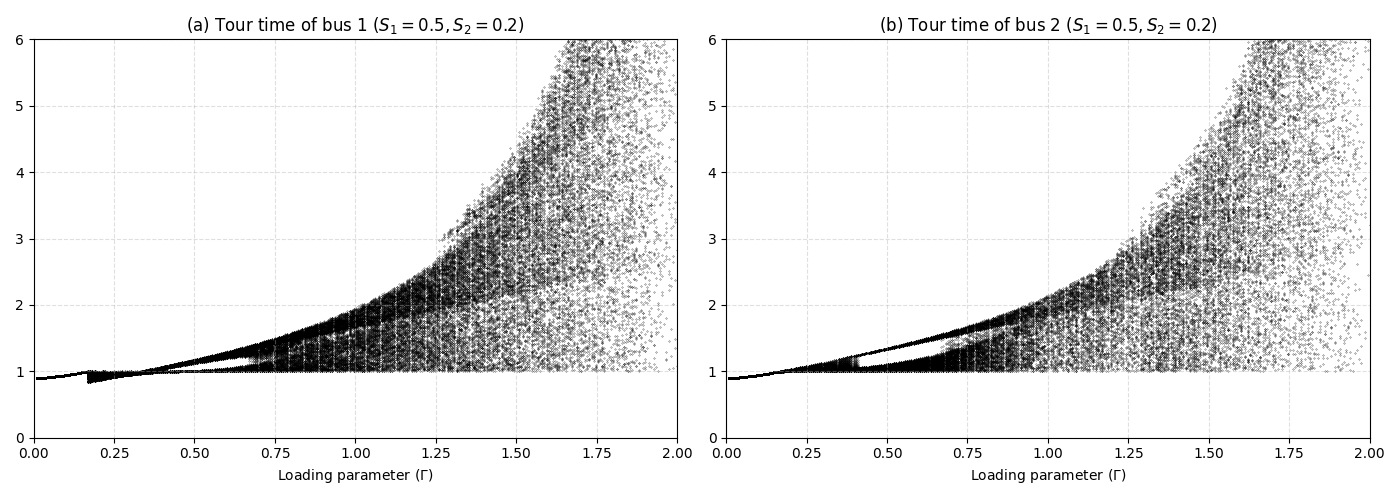
\includegraphics[width=\textwidth]{fig4_tour_time.png}
		\end{column}
		\begin{column}{0.5\textwidth}
			\centering
			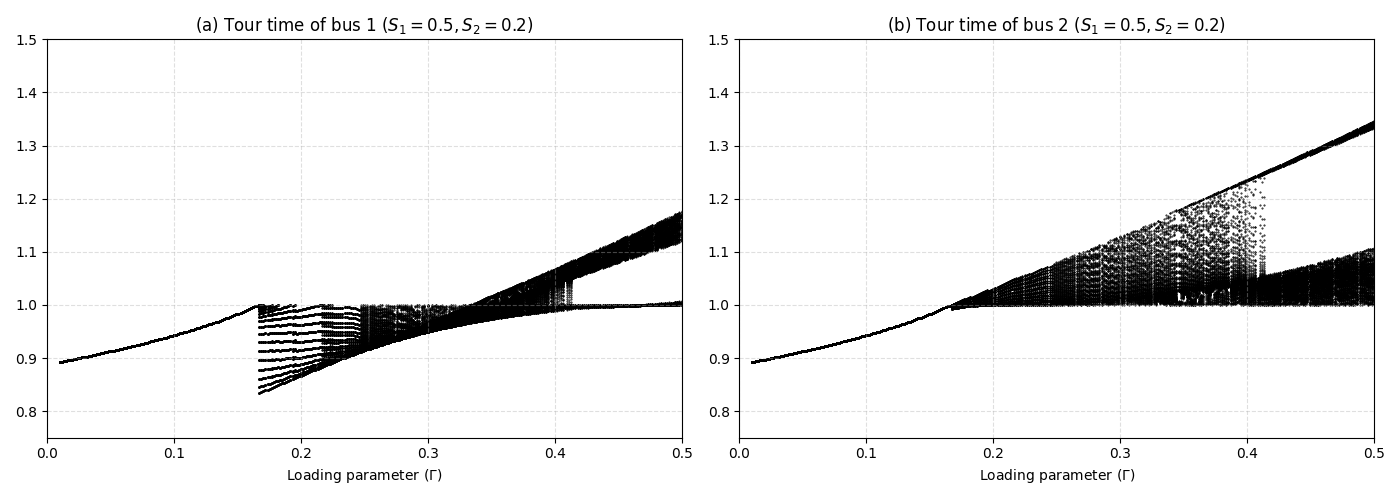
\includegraphics[width=\textwidth]{fig5_zoom.png}
		\end{column}
	\end{columns}

	\vspace{0.5em}
	Tour-time phản ánh trực tiếp headway qua bản đồ: khi headway dao động hỗn loạn, thời gian một chuyến đi-về cũng dao động bất thường -- ảnh hưởng trực tiếp đến \textbf{độ tin cậy lịch trình}.
\end{frame}

% =====================================================================
\useStyleLogoOnly
\useThickBar
\section{Kết quả: Phân tích không gian pha}
% =====================================================================

\begin{frame}{8. Return map hé lộ attractor}
	\begin{columns}[T]
		\begin{column}{0.55\textwidth}
			\centering
			
\includegraphics[width=0.95\textwidth]{fig6_return_map.png}
		\end{column}
		\begin{column}{0.45\textwidth}
			\begin{block}{Cách đọc return map}
				\begin{itemize}
					\item \textbf{Regular}: một điểm duy nhất (điểm cố định $\Delta^*$).
					\item \textbf{Periodic}: tập hợp hữu hạn điểm rời rạc (chu kỳ-$k$).
					\item \textbf{Chaotic}: một đường cong dày đặc -- dấu hiệu kinh điển của hỗn loạn xác định.
				\end{itemize}
			\end{block}
		\end{column}
	\end{columns}
\end{frame}

\begin{frame}{9. Thống kê Mean \& RMS}
	\begin{columns}[T]
		\begin{column}{0.55\textwidth}
			\centering
			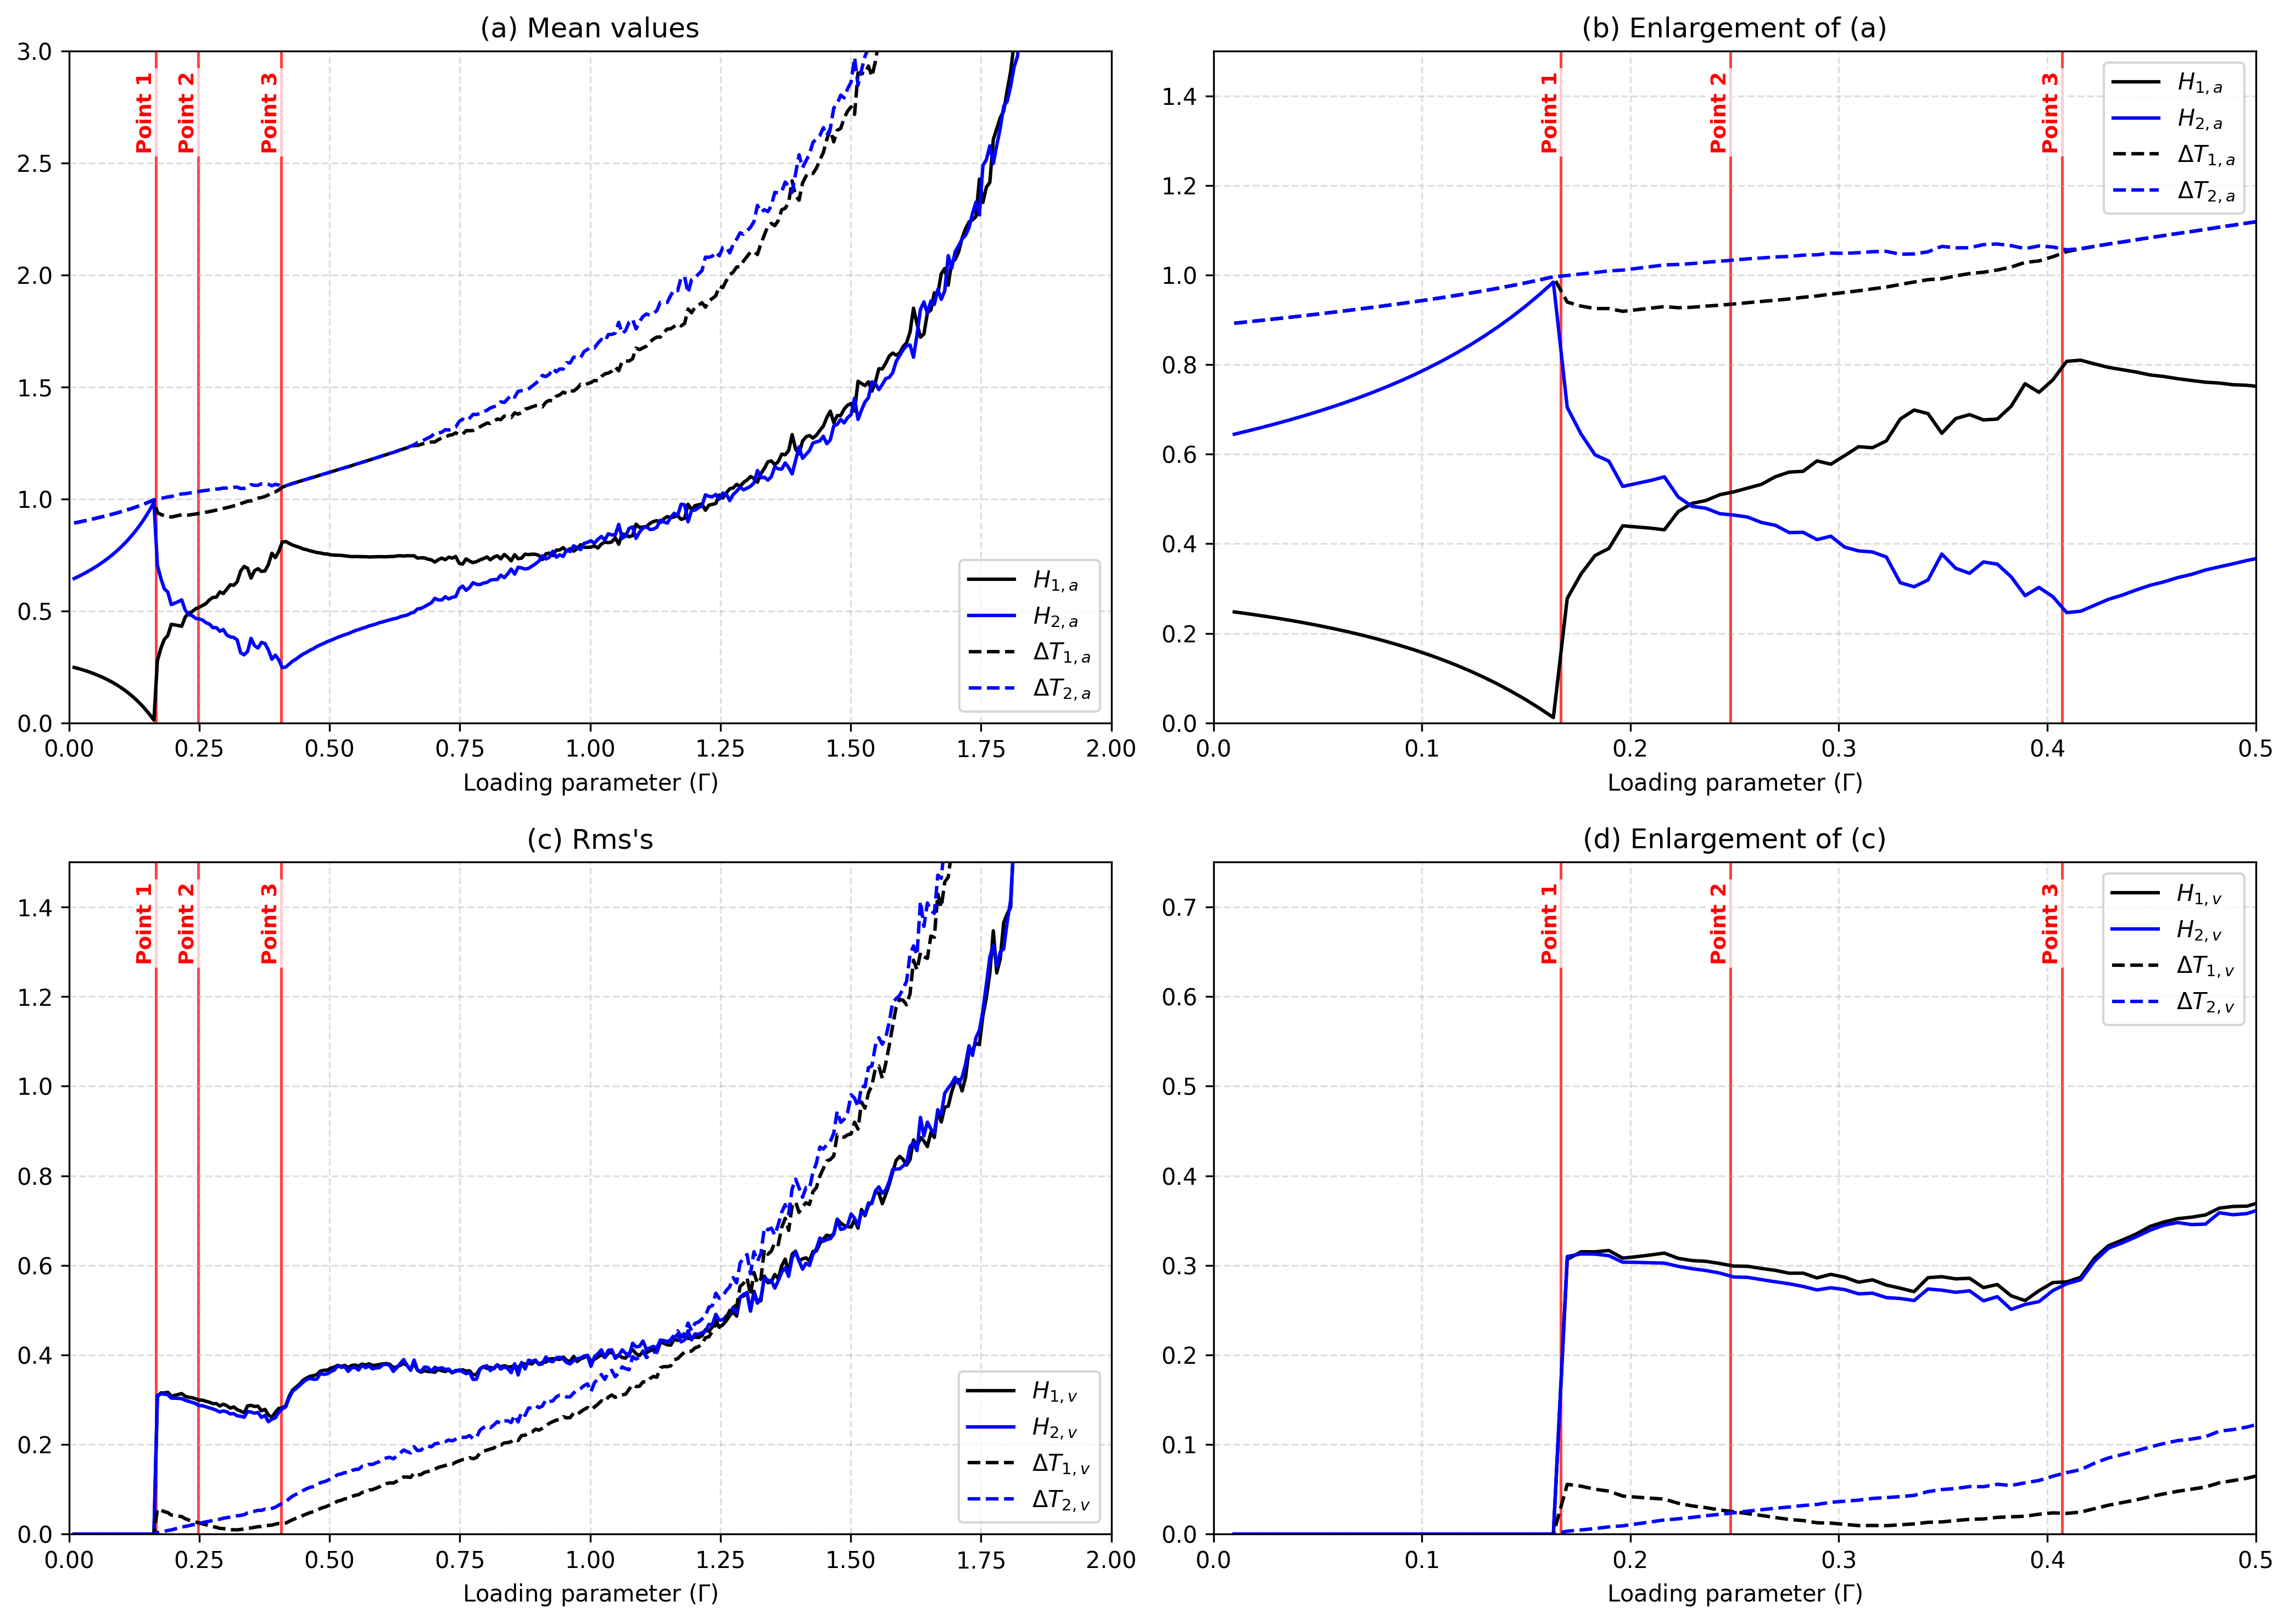
\includegraphics[width=0.95\textwidth]{fig7_mean_rms.png}
		\end{column}
		\begin{column}{0.45\textwidth}
			\begin{block}{Cách đọc đồ thị}
				\begin{itemize}
					\item \textbf{RMS $\approx 0$}: với $\Gamma$ nhỏ -- headway hội tụ về một giá trị không đổi (regular).
					\item \textbf{RMS tăng đột ngột}: tại $\Gamma=\Gamma^*$ -- khởi đầu dao động periodic/chaotic.
					\item \textbf{Mean tour-time} tăng nhanh khi $\Gamma \to 2$, báo hiệu sự sụp đổ.
				\end{itemize}
			\end{block}
		\end{column}
	\end{columns}

	\vspace{0.3em}
	\small Tiêu chí RMS này chính là cách ta dò \textbf{ngưỡng chuyển pha} $\Gamma^*(S)$ ở hình tiếp theo.
\end{frame}

\begin{frame}{10. Giản đồ pha (Phase Diagram)}
	\begin{columns}[T]
		\begin{column}{0.55\textwidth}
			\centering
			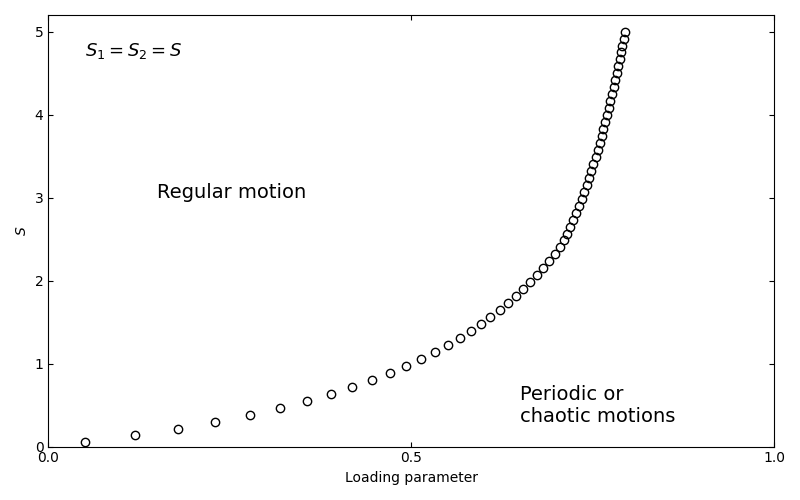
\includegraphics[width=0.95\textwidth]{fig8_phase_diagram.png}
		\end{column}
		\begin{column}{0.45\textwidth}
			\begin{block}{Hai miền động lực}
				Với mỗi giá trị tăng tốc $S=S_1=S_2$, có một ngưỡng tải tới hạn $\Gamma^*$ ngăn cách hai miền: \textbf{regular motion} ở dưới đường cong, và \textbf{periodic/chaotic motion} ở trên.
			\end{block}
			\begin{itemize}
				\item Đường biên tuân theo $\Gamma^*=\dfrac{S}{S+1}$.
				\item Đường cong tiến gần $\Gamma\to0.8$ khi $S\to\infty$, luôn nhỏ hơn $\Gamma=1$ với $S\le 5$.
			\end{itemize}
		\end{column}
	\end{columns}
\end{frame}

% =====================================================================
\useStyleHustFull
\useThinBar
\section{Khám phá tương tác}
% =====================================================================

\begin{frame}{11. Khám phá động lực học một cách tương tác}
	\textbf{Vì sao:} các hình tĩnh chỉ thể hiện một bộ tham số tại một thời điểm -- nhưng đặc điểm nổi bật nhất của hệ này là \emph{tốc độ thay đổi tính chất} khi $\Gamma$ và $S_i$ biến thiên.

	\vspace{0.5em}
	\textbf{Những gì công cụ thể hiện:}
	\begin{itemize}
		\item Thay đổi $\Gamma, S_1, S_2$ sẽ vẽ lại ngay các đồ thị headway, tour-time và return map, đặt cạnh nhau.
		\item Một khung nhìn bifurcation quét liên tục $\Gamma$, cho thấy chuỗi chuyển đổi regular $\to$ periodic $\to$ chaotic trong một hình duy nhất.
		\item Giản đồ pha có thể được dựng lại trực tiếp, vẽ đường biên $\Gamma^*(S)$ theo thời gian thực.
	\end{itemize}

	\vspace{0.5em}
	Nhờ vậy, quá trình chuyển pha trong giản đồ pha không còn là một hình tĩnh, mà là điều người xem có thể quan sát diễn ra trực tiếp.
\end{frame}

% =====================================================================
\section{Kết luận}
% =====================================================================

\begin{frame}{12. Kết luận \& hướng mở rộng}
	\begin{block}{Những gì đã tìm thấy}
		\begin{itemize}
			\item Chỉ một quy tắc phản hồi đơn giản -- "khách đông $\to$ xe chạy nhanh hơn" -- đủ để biến một lịch trình xe buýt hoàn toàn đều đặn thành hỗn loạn.
			\item Sự chuyển đổi này chỉ bị chi phối bởi hai tham số $\Gamma$ và $S$, với một đường biên rõ ràng $\Gamma^*=S/(S+1)$ giữa regular motion và motion bất thường.
			\item Vượt qua $\Gamma=2$, hệ không còn điểm vận hành ổn định nào: tour-time phân kỳ.
		\end{itemize}
	\end{block}

	\begin{alertblock}{Ý nghĩa \& hướng mở}
		Giảm $\Gamma$ hoặc điều chỉnh $S_i$ có thể giữ hệ xe buýt trong miền regular -- một chiến lược điều khiển đơn giản và khả thi. Hướng mở rộng tự nhiên: \textbf{xe không đối xứng} ($S_1 \neq S_2$) và \textbf{nhiều hơn hai xe}, để xem hiện tượng dồn xe có lan truyền trong một đội xe lớn hơn không.
	\end{alertblock}
\end{frame}

% =====================================================================
\useStyleLogoOnly
\setbeamertemplate{bibliography item}[text]

\begin{frame}[allowframebreaks]{Tài liệu tham khảo}
	\begin{thebibliography}{99}
		\bibitem{nagatani2006}
		T. Nagatani,
		``Chaos control and schedule of shuttle buses,''
		\emph{Physica A: Statistical Mechanics and its Applications}, vol. 371, no. 2, pp. 683--691, 2006.

		\bibitem{nagatanireview}
		T. Nagatani,
		``The physics of traffic jams,''
		\emph{Reports on Progress in Physics}, vol. 65, no. 9, pp. 1331--1386, 2002.
	\end{thebibliography}
\end{frame}

\hustcontactpage{\hfill CẢM ƠN \hfill}{
	\textbf{Nhóm 3} \\
	\textbf{Đề tài:} Hỗn loạn và điều khiển lịch trình xe buýt con thoi
	\vspace{0.5cm}

	\begin{itemize}
		\item Rất mong nhận được câu hỏi và trao đổi từ Hội đồng.
	\end{itemize}

	\vspace{1cm}
	\textit{Xin chân thành cảm ơn!}
}

\end{document}
